% !TeX root = RJwrapper.tex


\title{Supplementary Information \protect\\ \Large PINstimation: An R Package for Estimating Probability of Informed Trading Models}
\author{by Montasser Ghachem, and Oguz Ersan}
\maketitle

\listoftables
\listoffigures

% \address{Montasser Ghachem\\
%   Department of Economics, Stockholm University\\
%   Stockholm, 106 91, Sweden\\
%   Sweden\\
%   (0000-0001-6991-3316)\\
%   \email{montassar.ghachem@su.se}}

% \address{Oguz Ersan\\
%   International Trade and Finance Department, Kadir Has University\\
%   Istanbul, 34083\\
%   Turkey\\
%   (0000-0003-3135-5317)\\
%   \email{oguzersan@khas.edu.tr}}


\setcounter{table}{0}
\renewcommand{\thetable}{S\arabic{table}}

\setcounter{figure}{0}
\renewcommand{\thefigure}{S\arabic{figure}}

\begin{table}[H]
\caption{Slots of the \code{estimate.pin} object}
\label{tab:slots_estimatepin_object}
\footnotesize
\renewcommand{\arraystretch}{1.3}
\begin{tabular}{l|p{1.5cm}p{9cm}}
\toprule
\textbf{Slot} & \textbf{Type} & \textbf{Description} \\ 
\midrule
\code{success}& \code{logical} & returns \code{TRUE} if the estimation succeeded, \code{FALSE} otherwise. \\ 
\code{errorMessage}& \code{character} & returns an error message if the estimation has failed.\\
\code{convergent.sets}& \code{numeric} & returns the number of initial parameter sets, at which the likelihood function converged.\\
\code{algorithm}& \code{character} & returns the algorithm used to compute the initial parameter sets.\\
\code{factorization}& \code{character} & returns the factorization of the PIN likelihood function.\\
\code{parameters}&\code{list}& returns the list of the optimal estimates ($\alpha$, $\delta$, $\mu$, $\varepsilon_{b}$, $\varepsilon_{s}$)\\
\code{likelihood}&\code{numeric} & returns the value of the (factorization of the) likelihood function evaluated at the optimal set of parameters.\\
\code{pin}&\code{numeric} & returns the value of the probability of informed trading.\\
\code{pin.goodbad}& \code{list}& returns a list containing a decomposition of PIN into good-news, and bad-news PIN components. The decomposition has been suggested in \cite{Brennan2016Asymmetric}. The list has two elements: \code{pinG}, and \code{pinB} are the good-news, and bad-news components of PIN, respectively.\\
\code{dataset}&\code{dataframe}& returns the dataset of buys and sells used in the maximum likelihood estimation of the PIN model.\\
\code{initialsets}&\code{dataframe}& returns the initial parameter sets used in the MLE method.\\
\code{details}&\code{dataframe}& returns a data frame containing the ML-estimated parameters for each initial parameter set.\\
\code{runningtime}& \code{numeric} & returns the running time of the PIN estimation in seconds.\\
\bottomrule
\end{tabular}
\end{table}


\begin{table}[H]
\caption{Common slots of the \code{estimate.mpin} and \code{estimate.mpin.ecm} objects}
\label{tab:table_slots_estimatempin}
\renewcommand{\arraystretch}{1.3}
\footnotesize
\begin{tabular}{l|p{1.5cm}p{9cm}}
\toprule
\textbf{Slot} & \textbf{Type} & \textbf{Description} \\ 
\midrule
\code{success} & 
\code{logical} & 
returns \code{TRUE} if estimation succeeded, \code{FALSE} otherwise. \\  
\code{errorMessage} & 
\code{character} & 
returns an error message if the estimation has failed. \\  
\code{convergent.sets} & 
\code{numeric} & 
returns the number of initial parameter sets, at which the likelihood maximization converged. \\  
\code{method} & 
\code{character} & 
returns the estimation method used, and takes either: \code{"ML"} for Maximum-Likelihood estimation, or \code{"ECM"} for Expectation- conditional maximization algorithm. \\ 
\code{layers} & 
\code{numeric} & 
returns the number of layers detected in the trading data, estimated by the ECM algorithm, or provided by the user. \\  
\code{parameters} & 
\code{numeric} & 
returns the list of the optimal estimates \(\left(\boldsymbol{\alpha },\boldsymbol{\delta },\boldsymbol{\mu },\varepsilon_{b} , \varepsilon_{s}\right)\), where \(\boldsymbol{\alpha }\), \(\boldsymbol{\delta }\), and \(\boldsymbol{\mu }\) are numeric vectors of length layers. \\  
\code{likelihood} & 
\code{numeric} & 
returns the likelihood function evaluated at the optimal parameters. \\ 
\code{mpinJ} & 
\code{numeric} & 
returns the multilayer probability of informed trading per layer. \\  
\code{mpin} & 
\code{numeric} & 
returns the multilayer probability of informed trading. \\  
\code{mpin.goodbad} & 
\code{list} & 
returns a list containing a decomposition of MPIN into good-news, and bad-news MPIN components. The decomposition has been suggested for PIN measure in \cite{Brennan2016Asymmetric}. The list has four elements: \code{mpinG} (\code{mpinB}) is the global good-news (bad-news) component of MPIN, while \code{mpinGj} (\code{mpinBj}) is a vector containing the good-news (bad-news) component of MPIN computed per layer.\\  
\code{dataset} & 
\code{dataframe} & 
returns the dataset of buys and sells used in the maximum likelihood estimation of the MPIN model. \\  
\code{initialsets} & 
\code{dataframe} & 
returns the initial parameter sets used in the estimation.\\  
\code{details} & 
\code{dataframe} & 
returns a dataframe containing estimated parameters of the ML method /ECM algorithm for each initial parameter set.\\  
\code{aggregates} & 
\code{numeric} & 
returns an aggregation of information layer parameters: \(\alpha_{agg} = \sum_{j}^{}\alpha_{j}\), \( \delta_{agg}=\sum_{j}^{}\alpha_{j}\delta_{j}\), \( \mu_{agg} = \sum_{j}^{}\alpha_{j}\mu_{j}\), alongside \( \varepsilon_{b}\) and \( \varepsilon_{s}\). \\  
\code{runningtime} & 
\code{numeric} & 
returns the running time of MPIN estimation in seconds.\\  
\bottomrule
\end{tabular}
\end{table}



\begin{table}[H]
\caption{Additional slots of the \code{estimate.mpin.ecm} object}
\label{tab:table_slots_estimatempin_ecm}
\renewcommand{\arraystretch}{1.3}
\footnotesize
\begin{tabular}{l|p{1.5cm}p{9cm}}
\toprule
\textbf{Slot} & \textbf{Type} & \textbf{Description} \\  
\midrule
\code{optimal$^*$} & 
\code{logical} & 
returns \code{TRUE} if the number of layers is optimized, and \code{FALSE} otherwise. \\  
\code{AIC$^*$} & 
\code{numeric} & 
returns the value of Akaike information criterion (AIC). \\  
\code{BIC$^*$} & 
\code{numeric} & 
returns the value of Bayesian information criterion (BIC). \\  
\code{AWE$^*$} & 
\code{numeric} & 
returns the value of Approximate Weight of Evidence (AWE). \\  
\code{criterion$^*$} & 
\code{character} & 
returns the model selection criterion used to find the optimal estimate. \\  
\code{hyperparams$^*$} & 
\code{numeric} & 
returns the hyperparameters of the ECM algorithm, which are \code{minalpha}, \code{maxeval}, \code{tolerance}, and \code{maxlayers}. \\  
\bottomrule
\end{tabular}
\end{table}



\begin{table}[H]
\caption{Slots of the \code{estimate.adjpin} object}
\label{tab:table_slots_estimateadjpin_object}
\renewcommand{\arraystretch}{1.3}
\footnotesize
\begin{tabular}{l|p{1.5cm}p{9cm}}
\toprule
\textbf{Slot}& 
\textbf{Type}& 
\textbf{Description}\\
\midrule
\code{success}& 
logical& 
returns \code{TRUE} if estimation has succeeded, \code{FALSE} otherwise.\\
\code{errorMessage}& 
\code{character} & 
returns an error message if the estimation has failed.\\
\code{convergent.sets}& 
\code{numeric} & 
returns the number of initial parameter sets, at which the likelihood maximization converged.\\
\code{method}& 
\code{character} & 
contains a reference to the estimation method: \code{"ECM"} for expectation-maximization algorithm, and \code{"ML"} for standard maximum likelihood estimation.\\
\code{factorization}& 
\code{character} & 
contains a reference to the factorization of the likelihood function used: \code{"GE"} for the factorization in \cite{Ersan2022methodological}, and \code{"NONE"} for the original likelihood function in \cite{duarte2009why}.\\
\code{restrictions}& 
\code{numeric} & 
returns a binary list that contains the set of parameter restrictions on the original AdjPIN model in the estimated AdjPIN model. If not empty, the list contains one or multiple of the following four elements \code{\{theta, mu, eps, d\}}. When a given element takes the value \code{TRUE}, then the estimated model assumes that the values of corresponding parameters are equal. For instance: \(\theta  = \theta'\) if \code{theta = TRUE}, \(\varepsilon_{b} = \varepsilon_{s}\) if \code{eps = TRUE}, \(\mu_{b} = \mu_{s}\) if \code{mu = TRUE}, and \(\Delta_{b} = \Delta_{s}\) if \code{d = TRUE}. \\
\code{algorithm}& 
\code{character} & 
returns the implemented initial parameter set determination algorithm. \code{"GE"} is for \cite{Ersan2022methodological}, \code{"CL"} is for \cite{cheng2021improvements}, \code{"RANDOM"} for random initial parameter sets, and \code{"CUSTOM"} for custom initial parameter sets.\\
\code{parameters}& 
\code{numeric} & 
returns a numeric vector of maximum-likelihood estimates: \(\left\{ \alpha ,\delta ,\theta ,\theta^{'},\varepsilon_{b},\varepsilon_{s},\mu_{b},\mu_{s},\Delta_{b},\Delta_{s}\right\}\)\\
\code{likelihood}& 
\code{numeric} & 
returns the likelihood function value at optimal parameters.\\
\code{adjpin}& 
\code{numeric} & 
returns the adjusted probability of informed trading.\\
\code{psos}& 
\code{numeric} & 
returns the probability of symmetric order flow shock, i.e., the probability that any given trade happens during a shock to both the number of buyer-initiated and seller-initiated trades.\\
\code{dataset}& 
\code{dataframe}& 
returns the dataset of buys and sells used in the maximum likelihood estimation of the AdjPIN model.\\
\code{initialsets}& 
\code{dataframe}& 
returns the initial parameter sets used in the estimation.\\
\code{details}& 
\code{dataframe}& 
returns a dataframe containing the estimated parameters for each initial parameter set.\\
\code{hyperparams$^*$}& 
\code{list}& 
returns the hyperparameters of the ECM algorithm, which are \code{maxeval} (maximum number of iterations) and \code{tolerance} (threshold of convergence for the difference between two consecutive ECM-likelihood values).\\
\code{runningtime}& 
\code{numeric} & 
returns the running time of the AdjPIN estimation in seconds.\\
\bottomrule
\end{tabular}
\end{table}



\begin{table}[H]
\caption{Slots of the \code{estimate.vpin} object}
\label{tab:slots_estimatevpin_object}
\renewcommand{\arraystretch}{1.3}
\footnotesize
\begin{tabular}{l|p{1.5cm}p{9cm}}
\toprule
\textbf{Slot} & 
\textbf{Type} & 
\textbf{Description}\\ 
\midrule
\code{success} & 
\code{logical} & 
returns \code{TRUE} if estimation has succeeded, \code{FALSE} otherwise.\\ 
\code{errorMessage} & 
\code{character} & 
returns an error message if the estimation has failed.\\ 
\code{parameters} & 
\code{numeric} & 
returns a numeric vector of estimation parameters: \code{timebarSize} is the size of timebars in seconds; buckets is the number of buckets per daily average volume; \code{VBS} is Volume Bucket Size (daily average volume/ buckets); \code{samplength} is the window length used to estimate VPIN; and \code{\#days} is the number of days in the dataset.\\ 
\code{bucketdata} & 
\code{dataframe} & 
returns a dataframe with detailed information about buckets. We report for each bucket its identifier \code{bucket}, the aggregate buy (sell) volume \code{agg.bVol}(\code{agg.sVol}), the absolute order imbalance \code{AOI =}$\vert$\code{agg.bVol-agg.sVol}$\vert$, the start time (\code{starttime}), the end time (\code{endtime}), the duration in seconds (\code{duration}) as well as the VPIN vector. \\ 
\code{vpin} & 
\code{numeric} & 
returns the vector of the volume-synchronized probabilities of informed trading.\\ 
\code{dailyvpin} & 
\code{dataframe} & 
returns the daily Volume-Synchronized Probability of Informed Trading. It is calculated in two different ways: \code{dvpin}, the average of vpin values, and \code{dvpin.weighted}, the duration-weighted average of the vpins on any day.\\ 
\code{runningtime} & 
\code{numeric} & 
returns the running time of the VPIN estimation in seconds.\\
\bottomrule
\end{tabular}
\end{table}


\begin{table}[H]
\caption{Slots of the \code{data.series} object}
\label{tab:slots_dataseries_object}
\renewcommand{\arraystretch}{1.3}
\footnotesize
\begin{tabular}{l|p{1.5cm}p{9cm}}
\toprule
\textbf{Slot} & 
\textbf{Type} & 
\textbf{Description}\\ 
\midrule
\code{series} & 
\code{numeric} & 
returns the number of \code{dataset} objects stored.\\
\code{model} & 
\code{character} & 
returns the model being simulated: \code{"MPIN"} or \code{"adjPIN"}. \\
\code{days} & 
\code{numeric} & 
returns the length of the simulated data in days common to \code{dataset} objects stored. The default value is \code{60}. \\
\code{layers} & 
\code{numeric} & 
returns a vector of information layers in the different \code{dataset} objects.  \\
\code{datasets} & 
\code{list} & 
returns the list of the \code{dataset} objects stored.\\
\code{restrictions} & 
\code{list} & 
returns a binary list that contains the set of parameter restrictions on the original AdjPIN model in the estimated model. If not empty, the list contains one or multiple of the following four elements \code{\{theta, mu, eps, d\}}. When a given element takes the value \code{TRUE}, then the estimated model assumes that the values of corresponding parameters are equal. For instance: \(\theta  = \theta'\) if \code{theta = TRUE}, \(\varepsilon_{b} = \varepsilon_{s}\) if \code{eps = TRUE}, \(\mu_{b} = \mu_{s}\) if \code{mu = TRUE}, and \(\Delta_{b} = \Delta_{s}\) if \code{d = TRUE}. \\
\code{warnings} & 
\code{numeric} & 
returns numbers referring to the warning errors caused by a conflict between two arguments.\\
\code{runningtime} & 
\code{numeric} & 
returns the running time of the data simulation in seconds.\\
\bottomrule
\end{tabular}
\end{table}



\begin{table}[H]
\caption{Slots of the \code{dataset} object}
\label{tab:slots_dataset_object}
\renewcommand{\arraystretch}{1.2}
\footnotesize
\begin{tabular}{l|p{1.5cm}p{9cm}}
\toprule
\textbf{Slot} & 
\textbf{Type} & 
\textbf{Description}\\ 
\midrule
\code{model} & 
\code{character} & 
returns the model being simulated: \code{"MPIN"} or \code{"adjPIN"}. \\
\code{days} & 
\code{numeric} & 
returns the length of simulated data in days. The default value is \code{60}. \\
\code{layers} & 
\code{numeric} & 
returns the number of information layers in simulated data. The default is a number uniformly drawn from $\{1,\dots, 5\}$. \\
\code{theoreticals} & 
\code{list} & 
returns the list of the theoretical parameters used to generate the data. \\
\code{empiricals} & 
\code{list} & 
returns the list of the empirical parameters derived from generated data. \\
\code{aggregates} & 
\code{numeric} & 
returns an aggregation of information layers’ empirical parameters. The aggregate parameters are: \( \alpha_{agg} = \sum_{j}^{}\alpha_{j}\), \( \delta_{agg} = \sum_{j}^{}\alpha_{j}\delta_{j}\), \( \mu_{agg} = \sum_{j}^{}\alpha_{j}\mu_{j}\), alongside \( \varepsilon_{b}\) and \( \varepsilon_{s}\). \\ 

\code{emp.pin} & 
\code{numeric} & 
returns the PIN/MPIN/adjPIN value derived from the empirically estimated parameters of the generated data. \\

\code{likelihood} & 
\code{numeric} & 
returns the value of the likelihood function evaluated at the empirical parameters. \\

\code{data} & 
\code{dataframe} & 
returns a data frame containing the generated sequences of buyer-initiated and seller-initiated trades. \\

\code{restrictions} & 
\code{list} & 
returns a binary list that contains the set of parameter restrictions on the original AdjPIN model in the estimated model. If not empty, the list contains one or multiple of the following four elements \code{\{theta, mu, eps, d\}}. When a given element takes the value \code{TRUE}, then the estimated model assumes that the values of corresponding parameters are equal. For instance: \(\theta  = \theta'\) if \code{theta = TRUE}, \(\varepsilon_{b} = \varepsilon_{s}\) if \code{eps = TRUE}, \(\mu_{b} = \mu_{s}\) if \code{mu = TRUE}, and \(\Delta_{b} = \Delta_{s}\) if \code{d = TRUE}. \\
\code{warnings} & 
\code{character} & 
stores warning messages of conflicts between the function arguments. \\
\code{runningtime} & 
\code{numeric} & 
returns the running time of the data simulation in seconds.\\
\bottomrule
\end{tabular}
\end{table}

\begin{figure}[H]
    \centering
\begin{subfigure}[b]{0.8\textwidth}
    \centering
    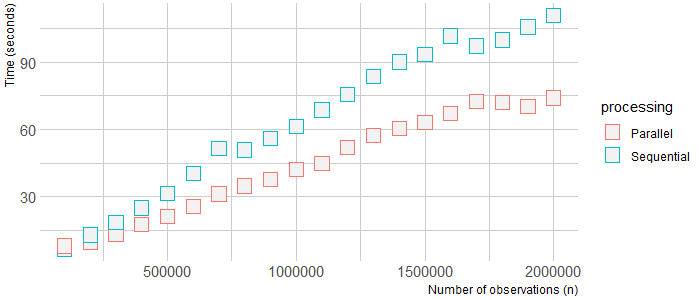
\includegraphics[width=\linewidth]{images/aggregate_complexity.png}
    \caption{Empirical time complexity of \code{aggregate\_trades()}}
    \label{subfig:complexity_aggregate}
  \end{subfigure}
  \begin{subfigure}[b]{0.8\textwidth}
    \centering
    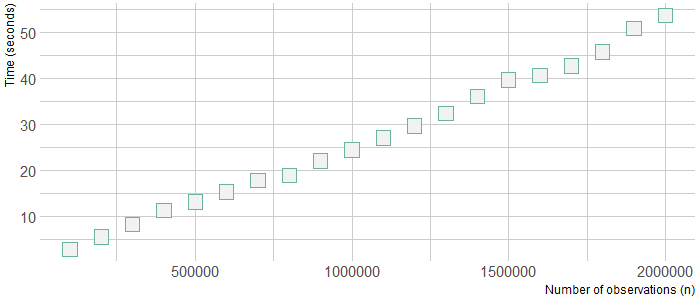
\includegraphics[width=\linewidth]{images/vpin_complexity.png}
    \caption{Empirical time complexity of \code{vpin()}}
    \label{subfig:complexity_vpin}
  \end{subfigure}
  \caption{Empirical time complexity of PINstimation functions}
\label{tab:time_complexity}
\end{figure}


% \begin{table}[H]
% \caption{Mean estimates of PIN and five parameters in PIN, MPIN, and ADJPIN models}
% \label{tab:apps_mean_estimates}
% \renewcommand{\arraystretch}{1.1}
% \setlength{\tabcolsep}{3pt}
% \small
% \begin{tabular}{p{2cm} p{2.2cm} p{1.1cm} p{1.1cm} p{1.1cm} p{1.2cm} p{1.2cm} p{1.2cm} p{1cm}}
% \toprule
% \multicolumn{9}{p{13.8cm}}{\footnotesize Table \ref{tab:apps_mean_estimates}: Mean values for estimates of PIN, and five model parameters, as well as average running time. Probability terms, PIN, \(\alpha\), and \(\delta\) are in percentage. The average running time (\textit{time}) is in seconds.}\\ \midrule
% \textbf{Models} & \textbf{Name} & \textbf{PIN} & \(\boldsymbol{\alpha }\) & \(\boldsymbol{\delta }\) & \(\boldsymbol{\mu }\) & \(\boldsymbol{\varepsilon }_{\boldsymbol{b}}\) & 
% \(\boldsymbol{\varepsilon }_{\boldsymbol{s}}\) & \textbf{Time}\\ 
% \midrule
% \multirow{3}{2pt}{PIN Models} 
% &\code{PIN\_EA}&13.316&17.871&29.45&984.833&727.163&709.545&1.344\\
% &\code{PIN\_GWJ}&13.385&18.352&30.171&960.139&731.366&706.103&0.291\\
% &\code{PIN\_YZ}&13.316&17.871&29.45&984.833&727.163&709.545&25.098\\
% % &\code{PIN\_YZ\_EA}&13.316&17.871&29.45&984.833&727.163&709.545&19.982\\
% % &\code{PIN\_EA\_LK}&13.316&17.871&29.45&984.833&727.163&709.545&1.334\\
% % &\code{PIN\_EA\_EHO}&7.273&23.043&29.881&157.523&830.819&751.281&1.452\\
% % &\code{PIN\_EA\_1}&13.035&17.479&31&990.869&727.449&709.478&0.267\\
% % &\code{PIN\_EA\_10}&13.316&17.871&29.45&984.833&727.163&709.545&2.635\\
% \midrule
% \multirow{3}{2pt}{MPIN Models} 
% &\code{MPIN.ML\_EG}&23.910&58.537&23.081&534.789&581.911&684.098&49.641\\
% &\code{MPIN.ML\_E}&20.972&47.633&21.701&528.856&619.009&695.322&23.84\\
% % &\code{MPIN.ML\_EM}&25.494&62.619&22.876&541.737&593.514&681.075&80.661\\
% &\code{MPIN.ECM}&22.461&54.513&24.563&515.325&665.626&689.832&67.179\\
% % &\code{MPIN.EM\_ALL}&22.239&54.077&24.565&516.202&664.323&689.757&161.672\\
% \midrule
% \multirow{4}{2pt}{ADJPIN Models} 
% &\code{ADJPIN\_GE}&12.658&40.836&48.91&642.788&610.051&554.048&12.449\\
% &\code{ADJPIN\_RND}&13.484&42.805&50.232&661.256&610.924&549.872&12.49\\
% &\code{ADJPIN.ECM\_GE}&12.282&40.641&47.496&627.301&632.203&564.216&2.589\\
% &\code{ADJPIN.ECM\_RND}&12.506&41.023&51.562&601.549&636.203&555.151&2.836\\
% % &\code{ADJPIN\_M1}&11.1&35.696&35.399&385.985&614.981&586.098&12.46\\
% % &\code{ADJPIN\_M2}&10.788&33.934&37.628&586.885&597.696&597.696&12.23\\
% % &\code{ADJPIN\_M3}&10.379&32.165&30.84&415.726&600.967&600.967&12.333\\
% \bottomrule
% \end{tabular}
% \end{table}



\begin{table}[H]
\caption{Conditional distributions of VPIN and positive/ negative post-returns}
\label{tab:table_distributions_vpinreturns}
\renewcommand{\arraystretch}{1.12}
\setlength{\tabcolsep}{3pt}
\setlength{\arrayrulewidth}{1pt}
\small
\begin{tabular}{p{1.2cm}p{1.2cm}p{1.2cm}p{1.2cm}p{1.2cm}p{1.2cm}p{1.2cm}p{1.2cm}p{1.2cm}p{1.2cm}}
\toprule
\multicolumn{10}{p{14cm}}{\footnotesize Table \ref{tab:table_distributions_vpinreturns} - The table provides distributions of either post-returns (Panels A, B) or VPIN values (Panels C, D); for positive (Panels A, C) and negative (Panels B, D) post-return observations separately. For brevity, only the 5\textsuperscript{th}, 50\textsuperscript{th} and 100\textsuperscript{th} quantiles are reported in each panel. Numbers are given in percentages. The table reports statistics  on \(29\) small cap, and \(29\) large cap stocks listed in NASDAQ Stockholm, for trading days in the last quarter of \(2020\). \(166,875\) VPIN observations are computed using the parameter set \code{(1-50-50)} implemented on \(5,410,411\) trades. However, zero return observations are excluded, leaving \(56,904\) positive, and \(57,301\) negative post-return observations.}\\
\midrule
\multicolumn{10}{p{14cm}}{\textbf{Panel A: Post-returns conditional on VPIN $\vert$ Positive returns}}\\
\midrule
&  0.25&  0.5&  0.75&  1&  1.25&  1.5&  1.75&  2&  >2.00\\
0.107&47.57&24.93&13.54&6.22&2.67&1.65&0.77&0.98&1.65\\
0.254&75.35&15.93&4.36&1.58&0.88&0.74&0.42&0.18&0.56\\
1&44.3&24.4&11.08&5.66&4.4&2.92&1.83&1.55&3.87\\
\midrule
\multicolumn{10}{p{14cm}}{\textbf{Panel B: Post-returns conditional on VPIN $\vert$ Negative returns}}\\
\midrule
&  -0.25&  -0.5&  -0.75&  -1&  -1.25&  -1.5&  -1.75&  -2&  <-2.00\\
0.1&47.5&26.84&12.34&5.98&2.92&1.91&0.73&0.56&1.22\\
0.253&76.7&16.17&3.41&1.39&1.01&0.38&0.28&0.14&0.52\\
1&43.88&22.57&12.45&7.06&3.72&2.92&2.12&0.97&4.31\\
\midrule
\multicolumn{10}{p{14cm}}{\textbf{Panel C: VPIN conditional on post-returns $\vert$ Positive returns}}\\
\midrule
&  0.25&  0.5&  0.75&  1&  1.25&  1.5&  1.75&  2&  >2.00\\
0.107&3.54&6.39&10.88&11.34&9.09&8.64&7.14&12.44&8.06\\
0.254&5.61&4.08&3.5&2.88&2.99&3.86&3.9&2.22&2.74\\
1&3.3&6.25&8.9&10.31&14.95&15.26&16.88&19.56&18.87\\
\midrule
\multicolumn{10}{p{14cm}}{\textbf{Panel D: VPIN conditional on post-returns $\vert$ Negative returns}}\\
\midrule
&  -0.25&  -0.5&  -0.75&  -1&  -1.25&  -1.5&  -1.75&  -2&  <-2.00\\
0.1&3.5&7.1&10.15&11.01&9.96&10.46&6.16&8.25&5.81\\
0.253&5.64&4.27&2.8&2.56&3.44&2.09&2.35&2.06&2.49\\
1&3.23&5.97&10.24&13&12.69&15.97&17.89&14.43&20.6\\
\bottomrule
\end{tabular}
\end{table}

\newpage
\bibliography{SI_pinstimation.bib}